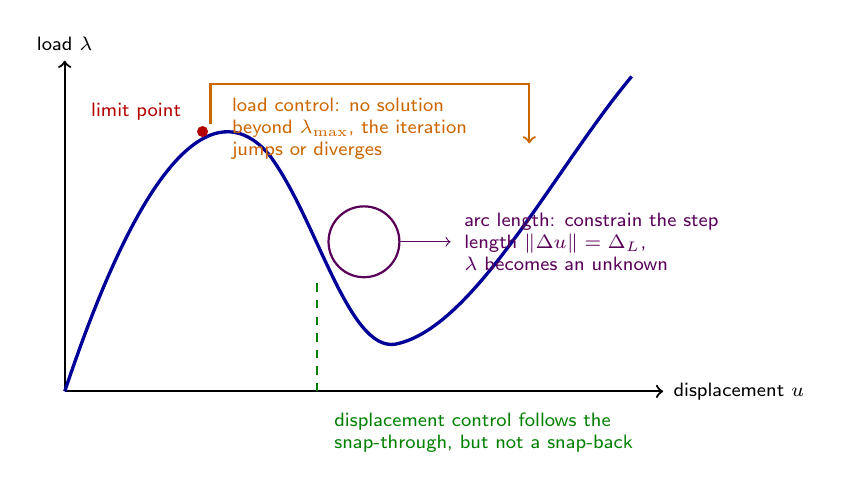
\begin{tikzpicture}[font=\sffamily\scriptsize]
\draw[->,thick] (0,0) -- (7.6,0) node[right] {displacement $u$};
\draw[->,thick] (0,0) -- (0,4.2) node[above] {load $\lambda$};
\draw[very thick,blue!60!black] (0,0) .. controls (1.2,3.6) and (2.1,3.6) .. (2.6,3.0) .. controls (3.2,2.2) and (3.6,0.5) .. (4.2,0.6) .. controls (5.2,0.8) and (6.2,2.8) .. (7.2,4.0);
\fill[red!70!black] (1.75,3.3) circle (2pt);
\node[red!70!black,anchor=east] at (1.6,3.55) {limit point};
\draw[orange!80!black,thick,->] (1.85,3.4) -- (1.85,3.9) -- (5.9,3.9) -- (5.9,3.15);
\node[orange!80!black,anchor=north west,align=left] at (2.0,3.85) {load control: no solution\\beyond $\lambda_{\max}$, the iteration\\jumps or diverges};
\draw[green!50!black,thick,dashed] (3.2,0) -- (3.2,1.4);
\node[green!50!black,anchor=north west,align=left] at (3.3,-0.15) {displacement control follows the\\snap-through, but not a snap-back};
\draw[violet!70!black,thick] (3.8,1.9) circle (0.45);
\draw[violet!70!black,->] (4.25,1.9) -- (4.9,1.9);
\node[violet!70!black,align=left,anchor=west] at (4.95,1.9) {arc length: constrain the step\\length $\|\Delta\bm u\|=\Delta_L$,\\$\lambda$ becomes an unknown};
\end{tikzpicture}
